\section{Implementation}

Since the first version of iFLUX, where we apply the \emph{lean} and \emph{agile} principles, we continued to apply these methodologies. Therefore, for the second version of iFLUX, we delivered feature after feature as fast as possible. We wanted to have something that we and others could experiment with rapidly, so that we would rapidly benefit from feedback. After few months, we have been able to implement a whole system with various demonstrators. We were able to assemble the different pieces by specifying rules. 

The very first user interface only provided a mechanism to create \emph{rules} and to simulate their evaluation. We have the possibility to enable the configuration of \emph{event sources} and \emph{action targets} as well. We now do most of our development on top of the Node.js platform, but we also SDKs in other languages.

\subsection{Architecture}

Since the project inception, we have relied on virtualization technologies, such as Vagrant and Docker, to make it easy for third-party developers to have a working environment on their machines. We introduced few technologies to let iFLUX be scalable. We introduced Kafka for the messaging bus letting the events be handled totally asynchronously. We received the events on a gateway dedicated to that and consume them on iFLUX rule engine. Therefore, a high charge of events will not be an issue as the cost to accept them is really small. We have also setup ElasticSearch to gain the possibility to use his full text capabilities. It is also an additional debug tool to see when and where the events comes and goes. You can refer to Figure \ref{fig:iflux-archi} to see the overall core architecture of the system.

\begin{figure}
\centering
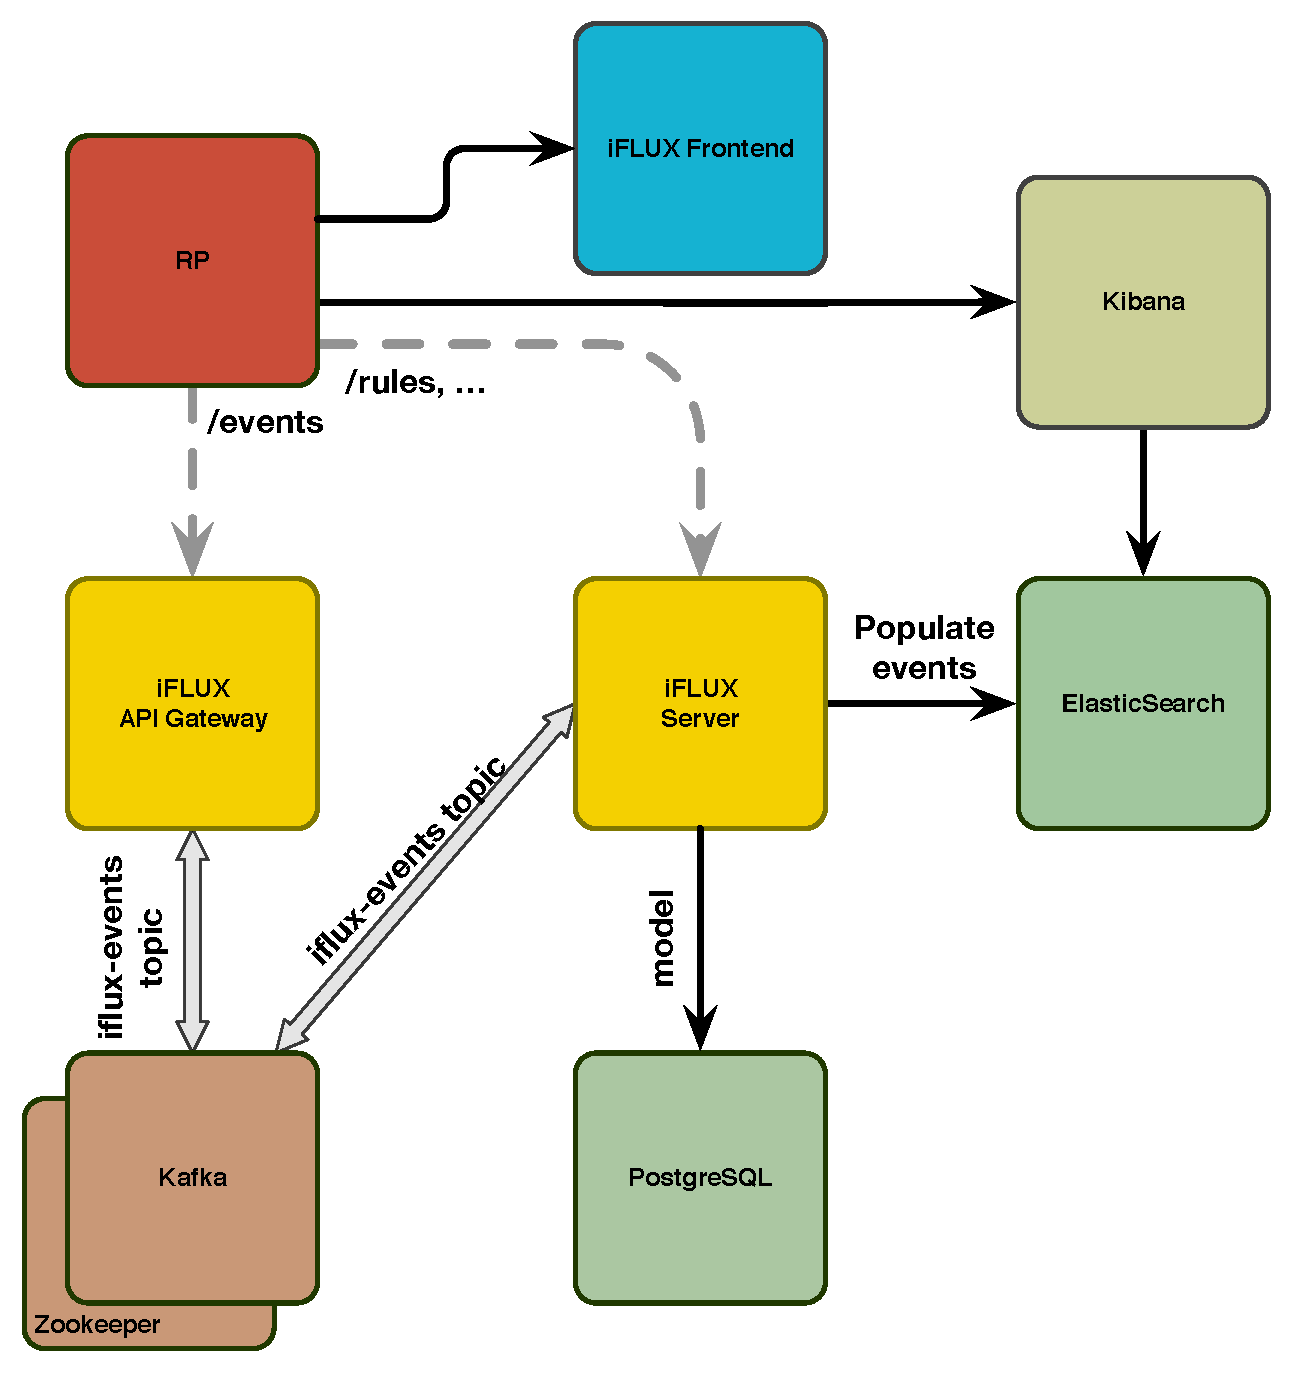
\includegraphics[width=1\columnwidth]{figures/iflux-archi.pdf}
\caption{The iFLUX architecture}
\label{fig:iflux-archi}
\end{figure}

\subsubsection{Reverse Proxy}

The reverse proxy receive all the inbound traffic and direct the requests to the right components. Kibana, iFLUX Frontend, iFLUX Gateway and iFLUX Server are accessible through the reverse proxy.

\subsubsection{iFLUX Frontend}

The frontend is the visual configuration tool of iFLUX. It offers CRUD operations through an Angular application to manipulate the iFLUX model. You can define event sources, action targets, rules and all required models.

\subsubsection{iFLUX API Gateway}

This gateway, today, offers only the \emph{/events/} API to accept quickly the events from the outside world without blocking any external system. This server is stateless and have no data store. The events received are forwarded to iFLUX Server through the message bus offered by Kafka.

\subsubsection{Kafka and Zookeeper}

We use Kafka to have a message bus to let the events to be handle asynchronously by the rule engine on the iFLUX Server. This component in the architecture let iFLUX to scale.

\subsubsection{iFLUX Server}

iFLUX Server manage the data models and has the rule engine. The rules are evaluated each time an event is received through the message bus. Once a rule is evaluated positively, action are triggered. But before an evaluation is done, the event received is stored in ElasticSearch for later analysis purpose. The result of the evaluation is also stored in ElasticSearch in a second index. The data model is stored in a PostgresSQL database.

\subsubsection{PostgresSQL}

Data backend of iFLUX. All the action targets, event sources, rules and so on are stored in this database. We do not store in this relational database any of the received events.

\subsubsection{ElasticSearch}

We use ElasticSearch to store the events and the result of the rules evaluation to make text searches and data analysis in the time. 

\subsubsection{Kibana}

Finally, Kibana is the frontend of ElasticSearch letting us to make text searches, to view graphs and trends on the events received and the evaluation results.

\subsection{REST APIs}

In addition of the three core abstraction of the iFLUX programming model, there are several additional resources exposed through the REST API. The endpoints are described in the following list: 

\begin{itemize}
\item \textbf{/auth} the authentication endpoint allow the users to register or sign in;
\item \textbf{/health} just an API to let the user to get the version of iFLUX core and to know the server is working;
\item \textbf{/actionTargets} where to manage the action targets;
\item \textbf{/actionTargetTemplates} where to manage the template of the action targets;
\item \textbf{/eventSources} where to manage the event sources;
\item \textbf{/eventSourceTemplates} where to manage the template of the event sources;
\item \textbf{/eventTypes} where to manage the event types;
\item \textbf{/me} where to get some info about himself;
\item \textbf{/organizations} where organization are managed. All in the iFLUX core is scoped to the organizations;
\item \textbf{/rules} where to manage the rules;
\item \textbf{/schemas} where to retrieve the JSON Schema used by the different iFLUX models;
\item \textbf{/events} not part of the iFLUX core directly as it is implemented on the gateway. But it is part of the general iFLUX API.
\end{itemize}

Apart from those endpoints, the event sources and the action targets, when required, must offer an API to configure the instances. On the action targets, an API to accept triggered action must be implemented.

\subsubsection{The \texttt{/events/} endpoint}

This endpoint and the payload that it accepts is straightforward. Every iFLUX \emph{event source} produces a stream of events. It POSTs these events on the endpoint. Notice that the payload accepts an array of events, so it is possible to send several events in a single request. For every event, there is a timestamp, a source (an ID to an event source), a type (a link to a JSON schema) and an array of custom properties. As you can see, writing an iFLUX event source is very simple. In particular, bringing an existing component (WoT gateway, mobile app, business application, etc.) into the iFLUX ecosystem is not a burden, which was one of our main design objectives. Furthermore, this can be done on any kind of platform (software and firmware), since the only requirement is to be able to issue an HTTP request.

\begin{lstlisting}
POST /events/ HTTP/1.1
Content-type: application/json

[
  {
    "timestamp" : "2015-01-12T05:21:07Z",
    "source" : "JI8928JFK",
    "type" : "http://localhost/eventTypes/temperatureEventSchema",
    "properties" : {
      "temperature" : 22.5,
      "location" : "room 1"
    }
  },
  {
    "timestamp" : "2015-01-12T05:22:07Z",
    "source" : "JI8928JFK",
    "type" : "http://localhost/eventTypes/temperatureEventSchema",
    "properties" : {
      "temperature" : 22.8,
      "location" : "room 1"
    }
  }
]
\end{lstlisting}

\subsubsection{The \texttt{/configure/} endpoint}

In the case of event source and action target that requires a dedicated configuration, iFLUX core will call the \texttt{/configure/} on the remote host. This remote endpoint should offer the API.

The action target must let the possibility to set an action target ID and a bunch of free properties.

\begin{lstlisting}
POST /configure/ HTTP/1.1
Content-type: application/json

{
  "target" : "8JFKJI892",
  "properties" : {
    "periodicity" : "daily"
  }
}
\end{lstlisting}

The event source must let the possibility to set an event source ID and a bunch of free properties.

\begin{lstlisting}
POST /configure/ HTTP/1.1
Content-type: application/json

{
  "source" : "JI8928JFK",
  "properties" : {
    "sensorId" : "thermo-1"
  }
}
\end{lstlisting}

\subsubsection{The \texttt{/actions/} endpoint}

This endpoint is analogous to the events endpoint. It has to be implemented by every \emph{action target}, to expose functionality that can be triggered when iFLUX rules are evaluated positively. Here again, it is possible to send several action payloads in a single HTTP request. Every action has a type (a link to a JSON schema) and a list of custom properties that depend on this type. Notice that there is no link to the action target, since this information is already part of the action resource URL (e.g. \url{https://myactuator.mysystem.com/actions/}). It must also contains the action target ID to identify which instance will be triggered. In case the action target is not configurable, the action target ID is sent anyway but should be skipped.

\begin{lstlisting}
POST /actions/ HTTP/1.1
Content-type: application/json

[
  {
    "target": "8JFKJI892",
    "type" : "http://localhost/actionTypes/sendAlertViaEmailSchema",
    "properties" : {
      "email" : "user.name@iflux.io",
      "subject" : "Alert: something has happened!",
      "body" : "An event has been notified to iFLUX by a source and a rule states that we should inform you about it."
    }
  },
  {
    "target": "8JFKJI892",
    "type" : "http://localhost/actionTypes/sendAlertViaEmailSchema",
    "properties" : {
      "email" : "user.name@iflux.io",
      "subject" : "Alert: something has happened!",
      "body" : "An event has been notified to iFLUX by a source and a rule states that we should inform you about it."
    }
  }
]
\end{lstlisting}

\subsubsection{The \texttt{/rules/} endpoint}

This endpoint is used to perform CRUD operations of iFLUX rules. Unlike the previous endpoints, which only accept POST requests, it accepts GET, POST, PATCH and DELETE requests. In addition to the simple metadata (a description and a reference), every rule has two parts: the \emph{conditions} part and the \emph{transformations} part. The \emph{conditions} part specifies under which conditions the rule will be fired. It is possible (but not mandatory) to specify an event source, an event type and a list of property values. In other words, it is possible to define rules that are fired ``\emph{if any sensor sends an event with a temperature above 30 degrees}" or ``\emph{if the particular sensor in my kitchen sends any kind of event}". The \emph{transformations} part specifies which action(s) should be triggered on which \emph{action target(s)} when the rule is fired. The property \texttt{actionSchema} contains a javascript expression, which specifies how to create the action payload based on the event properties.

\begin{lstlisting}
POST /actions/ HTTP/1.1
Content-type: application/json

{
  "description" : "When a temperature event is received, notify Bob by email.",
  "reference": "TEMPERATURE-EMAIL-NOTIFICATION",
  "enabled": true,
  "conditions" : [{
    "eventSourceId" : 12,
    "eventTypeId" : 1
  }]
  "transformations" : [{
    "actionTargetId" : 28,
    "fn": {
    	"expression": "return { "temp": event.properties.temperature };"
    }
  }]
}\end{lstlisting}

\subsubsection{The other endpoints}

The GitHub repositories of iFLUX contains the API documentation which is more complete than the description given in this document. You should take a look on \url{https://github.com/SoftEng-HEIGVD/iflux-apidoc} or \url{https://iflux.heig-vd.ch/doc/} to have a deeper view on the APIs. You will realize that most of the APIs are CRUD oriented.

\subsection{The data model}

In iFLUX, we manipulate various data stored in a PostgreSQL database. The data stored are only related to the rules. No event is stored directly in iFLUX. In place, for the events, we rely on on ElasticSearch.

The Figure \ref{fig:data-model} presents the different models. In fact, this is really similar to the APIs. We have the organizations to scope all the data visibility to only members of the organizations. Action target and their templates like the event sources and their templates can be public or not. When they are defined as public, they become usable by every iFLUX registered users. Changing the visibility of any of this model will only prevent them to be used in the future. In figure, the dashed lines will refer to weak links meaning that the link is defined only in the code and not through database integrity constraints.

\begin{figure}
\centering
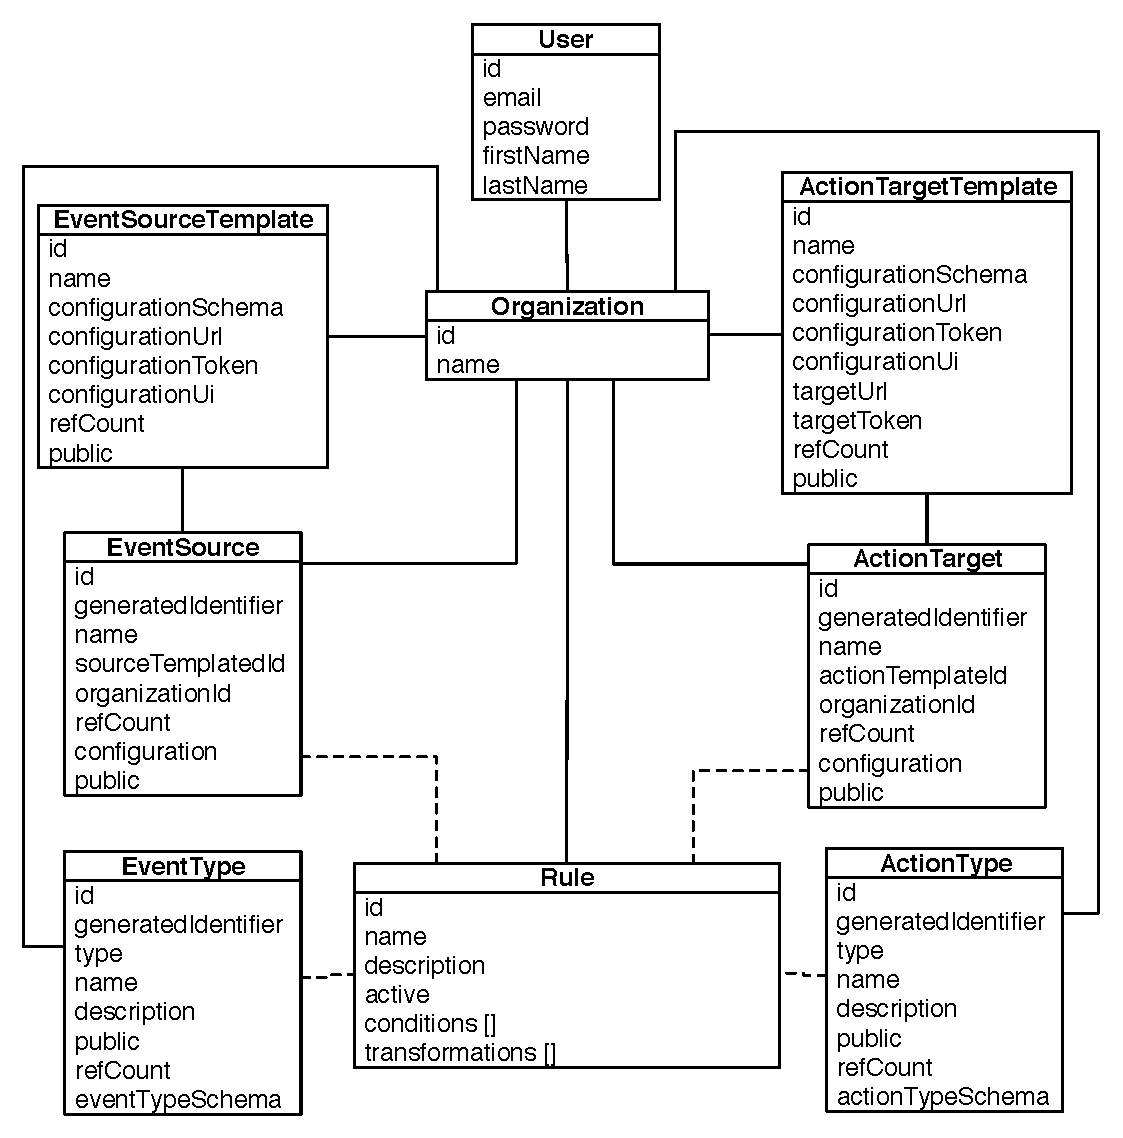
\includegraphics[width=1\columnwidth]{figures/data-model.pdf}
\caption{The iFLUX data model}
\label{fig:data-model}
\end{figure}

\subsubsection{Commons attributes}

In the next few sections, we will describe the different models of iFLUX. Some of them share the same attributes dedicated to the same usage. Therefore, we will describe them below:

\begin{itemize}
\item \textbf{generatedIdentifier} This a unique string across a model generated on the server side which is not editable by iFLUX users;
\item \textbf{refCount} this field is a cache of the number of times the model is referenced by another model. This is a shortcut to let the UI knowing if the model can be deleted or not;
\item \textbf{*Schema} in general, all the attributes terminated by the suffix Schema refers to a JSON Schema;
\item \textbf{*Token} when we talk about tokens in our models, this means that we expect a token that will be used in the HTTP header \emph{authentication} with a sort of \emph{bearer}; It is not yet possible to specify other security authentication schemes;
\item \textbf{public} when public flag is present, it means that the model can be kept private when set to false and therefore the model remains visible only by members of the same organization. If set to true, the model is visible by everybody in iFLUX. Only members of an organization can edit/delete models owned by the organization even if they are public.
\end{itemize}

\subsubsection{Organizations}

The organization is the main model in iFLUX. All the remaining data are scoped to the organizations. There is no way to transfer a model from an organization to another organization. In place of that, we have a public/private mechanism which allows to open the usage (not the edition) to everyone.

An organization is defined by a name that must be unique across the system.

\subsubsection{Users}

Users are automatically a member of at least one organization. There is no concept of privileges in an organization. Being part of an organization will allow the member to do everything in the organization. This means that any member can create, read, update or delete any model attached to the organization where the user is a member.

A user is defined by a first name, a last name and an email. In addition, the user has to set a password that will be stored ciphered in the database.

\subsubsection{Event Source Templates}

The event source templates define an event source that can be instantiated multiple times in the system. Refers to \ref{sec:est} for more details.

An event source template is composed of a name that is unique in the organization, a configuration schema. This schema define the JSON payload that the external system expect when the configuration callback is used. An optional configuration token can be set. In addition, a configuration UI schema is defined optionally to offer the possibility of the frontend to prepare a corresponding UI to make the configuration. Finally, they are ref count and public attributes.

\subsubsection{Event Sources}

Event sources are instances of event source templates. This will allow to define multiple event sources on the same model. For instance, you define an event source template to be a thermometer which can send temperature events. Then, you can define one or more real thermometers uniquely identified. Fore more details, check the section \ref{sec:es}.

An event source have a name that is unique across the event sources scoped to the organization. A reference to the event source template and an organization. The configuration is the real values that will be used to configure the instance of the event source template in the remote system. Finally, the attributes generated identifier, public and ref count are present.

\subsubsection{Event Types}

The event types define the structure of the events that an event source will produce. They are used to specify the data send from an event source and then letting the definition of rules to know which data available in the action.

An event type has a name that is unique across the organization and human description is possible. The event type schema is the format of events from that type. The type is the URL to refer the schema. If the URL refer to an external service, the schema can be blank. The attributes public, ref count and generated identifier are present.

\subsubsection{Action Target Templates}

The action target templates define an action target that can be instantiated multiple times in the system. Refers to \ref{sec:att} for more details.

An action target template is composed of a name that is unique in the organization, a configuration schema. This schema define the JSON payload that the external system expect when the configuration callback is used. An optional configuration token can be set. In addition, a configuration UI schema is defined optionally to offer the possibility of the frontend to prepare a corresponding UI to make the configuration. In addition, a target URL and its optional token is required for the action callbacks which is different from the configuration callback. Finally, they are ref count and public attributes.

\subsubsection{Action Targets}

Action targets are instances of action target templates. This will allow to define multiple action targets on the same model. For instance, you define an action target template to be a light which can send be switched on/off. Then, you can define one or more real lights uniquely identified. Fore more details, check the section \ref{sec:at}.

An action target have a name that is unique across the action targets scoped to the organization. A reference to the action target template and an organization. The configuration is the real values that will be used to configure the instance of the action target template in the remote system. Finally, the attributes generated identifier, public and ref count are present.

\subsubsection{Action Types}

The action types define the structure of the actions sent to action targets. It will help to define rules with the correct action data format in the JavaScript expressions.

An action type has a name that is unique across the organization and human description is possible. The action type schema is the format of actions from that type. The type is the URL to refer the schema. If the URL refer to an external service, the schema can be blank. The attributes public, ref count and generated identifier are present.

\subsubsection{Rules}

The rules do the relations between the event sources and the actions targets as it was explained section \ref{sec:rules}.

A rule is defined by a unique name across the organization and an optional human description. The active flag is used to enable/disable the evaluation of a rule.The conditions and transformations arrays are JSON arrays stored directly in the model. Therefore, there is no strong links with integrity constraints. 

The conditions is a list of \emph{if} with the following data structure. Only one condition evaluated to true is enough to match the rule.

\begin{lstlisting}
"properties": {
  "description": {
    "description": "Human friendly text to explain the condition.",
     "type": "string"
  },
  "eventSourceId": {
    "description": "Reference to event source. If blank, * is used.",
    "type": "integer"
  },
  "eventTypeId": {
    "description": "Reference to event type. If blank, * is used",
    "type": "integer"
  },
  "fn": {
    "description": "JavaScript expression. Can be blank.",
    "type": "object",
    "properties": {
      "expression": {
        "description": "MUST be a valid JavaScript expression",
        "type": "string"
      },
      "sampleEvent": {
        "description": "A valid event to be evaluated to true with the expression.",
        "type": "object"
      }
    },
    "required": [ "expression", "sample" ]
  }
}
\end{lstlisting}

and an example:

\begin{lstlisting}
"conditions": [{
  "description": "Match if a temperature has changed.",
  "eventSourceId": 1,
  "eventTypeId": 1,
  "fn": {
    "expression": "return event.temperature.old != event.temperature.new;",
    "sampleEvent": {
      "temperature": {
        "old": 12,
        "new": 13
      }
    }
  }
}]
\end{lstlisting}

The transformations is a list of \emph{then} with the following data structure. All the transformations will be applied.

\begin{lstlisting}
"properties": {
    "description": {
      "description": "Human friendly text to let the possibility to explain the transformation.",
      "type": "string"
    },
    "actionTargetId": {
      "description": "Reference to action target.",
      "type": "integer"
    },
    "actionTypeId": {
      "description": "Reference to action type.",
      "type": "integer"
    },
    "fn": {
      "description": "JavaScript expression to create the action content.",
      "type": "object",
      "properties": {
        "expression": {
          "description": "MUST be a valid javascript expression",
          "type": "string"
        },
        "sample": {
          "description": "A valid context to evaluate the transformation",
          "type": "object",
          "properties": {
            "event": {
              "description": "A valid event.",
              "type": "object"
            },
            "eventSourceTemplateId": {
              "description": "A reference to the event source template. Can be blank.",
              "type": "integer"
            },
            "eventTypeId": {
              "description": "A reference to the event type. Can be blank.",
              "type": "integer"
            }
          },
          "required": [ "event" ]
        }
      },
      "required": [ "expression", "sample" ]
    }
  },
  "required": [ "actionTargetId", "actionTypeId" ]
}
\end{lstlisting}

and an example:

\begin{lstlisting}
"transformations": [{
  "description": "Prepare a message for Slack with the old and new temperature",
  "actionTargetId": 1,
  "eventTypeId": 1,
  "actionTypeId": 1,
  "fn": {
    "expression": "return { message: 'The temp. changed from ' + event.temperature.old + ' to ' + event.temperature.new + '.' };",
    "sample": {
      "event": {
        "temperature": {
          "old": 12,
          "new": 14
        }
      },
      "eventSourceTemplateId": 1
    }
  }
}]
\end{lstlisting}

\subsection{Model summary}

In fact, the data model of iFLUX is not so complex. A lot of things that are present for the event side are also present in the action side. Only few details change between them. The logic behind this is that it is more easy to maintain and to factorize the code if the things are close. The difference between event and action sides is mainly due to the fact that the event side is an input stream in iFLUX and the action side is an output stream. Then, the action side models require more configuration than event side.



















